\documentclass[border=4pt,12pt]{standalone}
% House style for redrawn exam diagrams (diagram-v4: 0.4pt lines, filled -latex arrows, fine dashes; stipple and hatching drawn as real dots/lines (no PDF/SVG patterns, so they render in every browser and at any scale); transparent background). Every figure \input's this.
\usepackage{amsmath,amssymb}
\usepackage{txfonts}
\usepackage{pdfrender,xcolor}
% \halo{text}: label on shading. The shading stops just around each letter's outline (a thin knock-out that follows the
% glyphs, like the papers' typesetting), never a box. Owner: "I don't want a box around the text".
\newcommand{\halo}[1]{\leavevmode\rlap{\pdfrender{TextRenderingMode=2,LineWidth=2.2pt,LineJoinStyle=1,StrokeColor=white,FillColor=white}#1}#1}
\usepackage{tikz,pgfplots}
\pgfplotsset{compat=1.18}
\usetikzlibrary{arrows.meta,calc,angles,quotes,patterns,patterns.meta,intersections,positioning,decorations.markings,shapes.geometric}
% Stipple and hatching are drawn as actual dots / lines clipped to the region (path picture), NOT as pattern fills:
% SVG <pattern> fills vanish or blur when browsers scale the image, so the owner could not see the shading.
% Each dot is a 0.72pt square (keeps SVGs small; reads as a dot at print size). Dots sit on one global staggered grid, so neighbouring regions line up.
\makeatletter
\newdimen\ex@x \newdimen\ex@y \newdimen\ex@xa \newdimen\ex@ya \newdimen\ex@xb \newdimen\ex@yb \newcount\ex@row
\def\exam@stipplecolor{black!75}\def\exam@dotr{0.42pt}\def\exam@dotgap{2.5}
\def\ex@rowdots{\ifdim\ex@x<\ex@xb \pgfpathrectangle{\pgfqpoint{\dimexpr\ex@x-0.36pt\relax}{\dimexpr\ex@y-0.36pt\relax}}{\pgfqpoint{0.72pt}{0.72pt}}\advance\ex@x by \exam@dotgap pt\relax\expandafter\ex@rowdots\fi}
\def\exam@stipple{%
  \pgftransformreset% dots are sized in real points even inside scaled pictures
  \pgfpointanchor{path picture bounding box}{south west}\ex@xa=\pgf@x \ex@ya=\pgf@y
  \pgfpointanchor{path picture bounding box}{north east}\ex@xb=\pgf@x \ex@yb=\pgf@y
  \pgfsetfillcolor{\exam@stipplecolor}\pgfmathsetmacro\ex@h{\exam@dotgap/2}%
  \pgfmathtruncatemacro\ex@r{floor(\ex@ya/\ex@h)-1}\ex@row=\ex@r\relax
  \ex@y=\ex@r\dimexpr\ex@h pt\relax
  \loop\ifdim\ex@y<\ex@yb
    \pgfmathtruncatemacro\ex@c{floor(\ex@xa/\exam@dotgap)-1}\ex@x=\ex@c\dimexpr\exam@dotgap pt\relax
    \ifodd\ex@row \advance\ex@x by \ex@h pt\fi
    \ex@rowdots
    \advance\ex@y by \ex@h pt \advance\ex@row by 1
    \ifnum\numexpr\ex@row-(\ex@row/4)*4\relax=0 \pgfusepath{fill}\fi% flush every 4 rows: bounded TeX memory, few clip copies in the SVG
  \repeat\pgfusepath{fill}}
\newdimen\ex@d
\def\exam@hatch#1{% #1 = 1 for /, -1 for \ ; lines 45 degrees, 3pt apart
  \pgftransformreset
  \pgfpointanchor{path picture bounding box}{south west}\ex@xa=\pgf@x \ex@ya=\pgf@y
  \pgfpointanchor{path picture bounding box}{north east}\ex@xb=\pgf@x \ex@yb=\pgf@y
  \ex@d=\dimexpr\ex@yb-\ex@ya\relax \ex@x=\dimexpr\ex@xa-\ex@d\relax
  \loop\ifdim\ex@x<\ex@xb
    \ifnum#1>0 \pgfpathmoveto{\pgfqpoint{\ex@x}{\ex@ya}}\pgfpathlineto{\pgfqpoint{\dimexpr\ex@x+\ex@d\relax}{\ex@yb}}%
    \else \pgfpathmoveto{\pgfqpoint{\ex@x}{\ex@yb}}\pgfpathlineto{\pgfqpoint{\dimexpr\ex@x+\ex@d\relax}{\ex@ya}}\fi
    \advance\ex@x by 4.24pt
  \repeat
  \pgfsetlinewidth{0.4pt}\pgfsetstrokecolor{black}\pgfusepath{stroke}}
\def\examstipple{\exam@stipple}\def\examhatch{\exam@hatch}\def\examsetstipplecolor#1{\def\exam@stipplecolor{#1}}\def\examsetdotgap#1{\def\exam@dotgap{#1}}
\makeatother
% (legacy pattern kept for old files)
% staggered stipple like the NESA papers' dotted shading
\pgfdeclarepatternformonly{exam stipple}{\pgfpointorigin}{\pgfqpoint{2.2pt}{2.2pt}}{\pgfqpoint{2.2pt}{2.2pt}}{%
  \pgfpathcircle{\pgfqpoint{0.55pt}{0.55pt}}{0.42pt}\pgfpathcircle{\pgfqpoint{1.65pt}{1.65pt}}{0.42pt}\pgfusepath{fill}}
\tikzset{
  every picture/.style={line width=0.6pt, >={Latex[length=2mm,width=1.3mm]}},
  curve/.style={line width=0.6pt},
  open arrow/.style={-{Latex[length=2mm,width=1.3mm]}},  % owner: filled -latex heads everywhere, no open chevrons
  aux/.style={dash pattern=on 2pt off 1.5pt, line width=0.6pt},
  shade/.code={\def\exA{#1}\def\exB{none}\ifx\exA\exB\else\pgfkeysalso{fill=black!18}\fi},
  shade/.default=on,
  shade dots/.style={fill=none, path picture={\examstipple}},
  stipple color/.code={\examsetstipplecolor{#1}},
  stipple gap/.code={\examsetdotgap{#1}},
  shade dense dots/.style={fill=none, stipple gap=1.6, path picture={\examstipple}},
  shade hatch/.style={fill=none, path picture={\examhatch{1}}},
  shade hatch reverse/.style={fill=none, path picture={\examhatch{-1}}},
  shade solid/.style={fill=black},
  pt/.style={circle, fill, inner sep=1.1pt},
  open pt/.style={circle, draw, fill=white, inner sep=1.1pt},
}
\pgfplotsset{
  exam axes/.style={axis lines=middle, axis line style={->}, xlabel={$x$}, ylabel={$y$},
    xlabel style={anchor=west}, ylabel style={anchor=south}, tick label style={font=\small},
    every axis plot/.append style={line width=0.6pt, black}, samples=200, clip=false,
    enlargelimits=false, axis on top},
}

\begin{document}
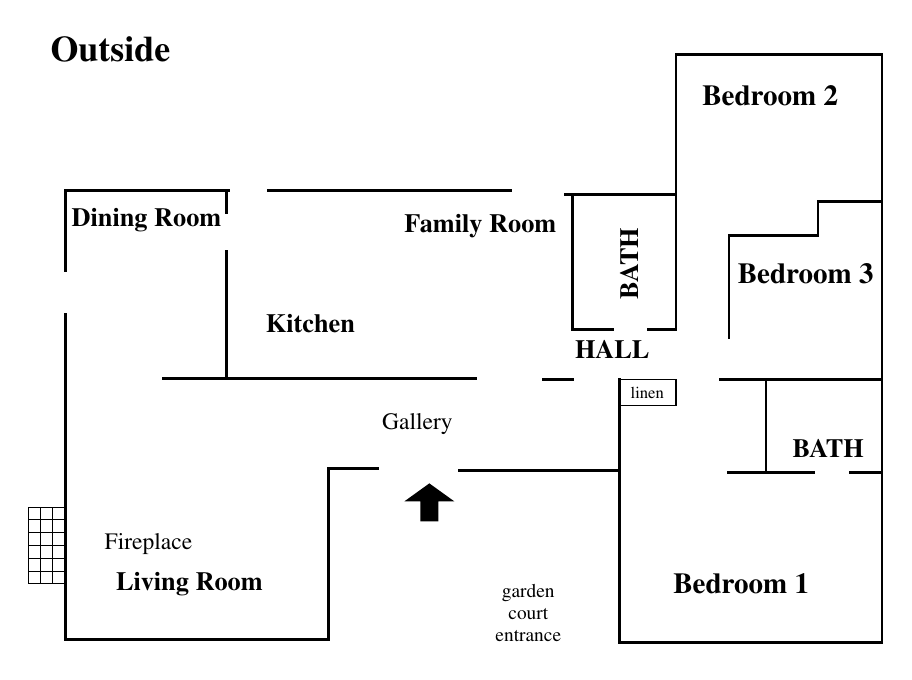
\begin{tikzpicture}[x=0.0127cm, y=-0.0127cm, wall/.style={line width=0.9pt, line cap=rect},
  room/.style={font=\bfseries\fontsize{9.5}{11}\selectfont, inner sep=0pt},
  big/.style={font=\bfseries\fontsize{10.5}{12}\selectfont, inner sep=0pt},
  small/.style={font=\fontsize{8.5}{10}\selectfont, inner sep=0pt}]
  % outer walls (crop pixel units; gaps are the openings shown on the plan)
  \draw[wall] (57,243) -- (57,163) -- (220,163);           % Dining: left wall top part, top wall
  \draw[wall] (218,163) -- (218,185);                      % stub beside the opening above the kitchen
  \draw[wall] (260,163) -- (502,163);                      % Kitchen / Family top wall
  \draw[wall] (557,167) -- (668,167);                      % top of the bathroom
  \draw[wall] (668,302) -- (668,27) -- (874,27) -- (874,615) -- (611,615) -- (611,352); % bedroom wing outline
  \draw[wall] (57,287) -- (57,612) -- (320,612) -- (320,441) -- (369,441);  % Living Room, courtyard side
  \draw[wall] (451,443) -- (611,443);                      % courtyard top wall (Gallery opens to the courtyard at the left)
  % inside walls
  \draw[wall] (218,224) -- (218,351);                      % Dining | Kitchen
  \draw[wall] (155,351) -- (467,351);                      % Kitchen/Family | Living/Gallery
  \draw[wall] (535,352) -- (564,352);                      % stub between Gallery and Hall
  \draw[wall] (564,167) -- (564,302) -- (604,302);         % bathroom left and bottom
  \draw[wall] (640,302) -- (668,302);
  \draw[wall] (721,310) -- (721,208) -- (810,208) -- (810,174) -- (874,174); % Bedroom 3 left and top
  \draw[wall] (712,352) -- (874,352);                      % Bedroom 3 bottom
  \draw[wall] (758,352) -- (758,445) -- (720,445);         % ensuite left wall
  \draw[wall] (758,445) -- (806,445); \draw[wall] (842,445) -- (874,445); % ensuite bottom, door to Bedroom 1
  % linen cupboard and fireplace
  \draw (611,352) rectangle (668,378); \node[font=\fontsize{6}{7}\selectfont] at (639,366) {linen};
  \draw (20,480) rectangle (57,556);
  \foreach \y in {492,505,518,531,544} \draw (20,\y) -- (57,\y);
  \foreach \x in {32,44} \draw (\x,480) -- (\x,556);
  % courtyard entrance arrow
  \fill (421,456) -- (446,474) -- (430,474) -- (430,494) -- (412,494) -- (412,474) -- (396,474) -- cycle;
  % labels
  \node[font=\bfseries\fontsize{13}{14}\selectfont] at (102,22) {Outside};
  \node[room] at (138,193) {Dining Room};
  \node[room] at (302,296) {Kitchen};
  \node[room] at (472,199) {Family Room};
  \node[room, rotate=90] at (621,236) {BATH};
  \node[room] at (604,322) {HALL};
  \node[big] at (762,68) {Bedroom 2};
  \node[big] at (797.5,246) {Bedroom 3};
  \node[room] at (820,421) {BATH};
  \node[small] at (409,397) {Gallery};
  \node[small] at (140,517) {Fireplace};
  \node[room] at (181,557) {Living Room};
  \node[big] at (733,556) {Bedroom 1};
  \node[font=\fontsize{7}{8}\selectfont, align=center] at (520,586) {garden\\court\\entrance};
\end{tikzpicture}
\end{document}
